%\begin{ndr}
%  This section should define all the external interfaces. This discussion should be based  on the system block diagram or context diagram to illustrate the relationship between this system and  other systems.
%\end{ndr}

\section{External interfaces}
The platform is  designed to be used through a front-end. This front-end provides several interfaces to use the platform.\\

\begin{center}
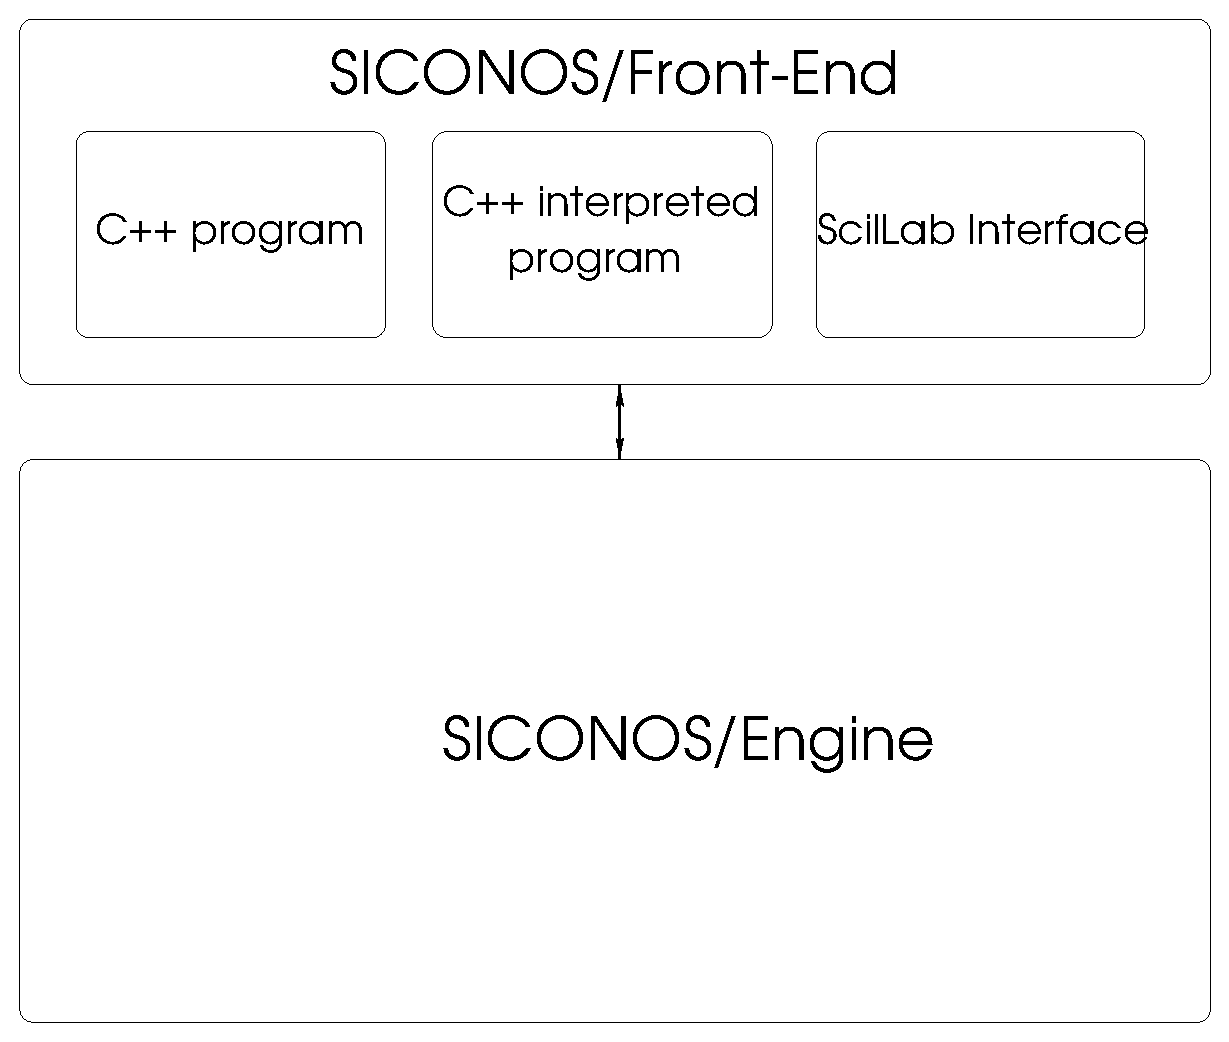
\includegraphics[scale=0.7]{figure/interfaces_scheme.eps}
\end{center}

\subsection{Native C++ interface: \acs{api} C++ }
The first interface will be written in C++. This \acs{api} C++ will contain :
\begin{itemize}
\item all of the public methods or functions of the \acs{engine}
\item a additional set of high level C++ methods in order to provide a macro language to drive the platform. 
\end{itemize}

This \ac{api} could be used in two different ways :
\begin{itemize}
\item compiled directly in an other application or a main file,
\item interpreted trough an C++ interpreter (e.g. Cint).
\end{itemize}


\subsubsection{Compiled C++ program}
%% \begin{ndr}
%% je n'etais pas d'accord avec ce qu'il y avait avant !!
%% le mecanisme d'acces dont vous parliez me semblait antinomique avec la notion
%% de programmation objet. Eventuellement on peut definir une classe debug qui soitami de tout et qui permette d'avoir une certaine visibilite mais ca reste du debug. En exploitation il faut imperativement respecter l'interface sinon c'est le bordel et alors autant faire du basic !
%% f. dubois
%% a completer
%% \end{ndr}

Following the definition of an \ac{api}, the user writes a program in C++, only using the public
functions/methods of \ac{frontend}. Then he must compile his program, and link it with the platform and finally run it to launch the simulation process.
During the execution of the program, it can access to the objects (attributes and methods) which are instantiated in the Engine only through the public interface. 

%\subsubsection{Interpreted C++ program}
%This way to launch a simulation is a little bit different from a compiled program. In fact, there is no compilation before running the program, but the program is only interpreted by an other program (Cint) which is linked with the platform. 

%An interpreted C++ program will have the same ability than a compiled C++ program.

\subsection{Interface with \acs{xxxlab}}
The interface through a scientific computation software will be the easiest way to use the computation platform. For example in
\ac{scilab}, the library corresponding to the platform would have to be loaded, and then the high level functions are available to the user.

\ac{scilab} will use functions especially designed for this software. That is to say some functions and objects of the \ac{engine} will
be created and used by calling high level functions which will be known by \ac{scilab}.

This type of interface will produce finally \ac{xxxlab} toolboxes.
